\chapter{Дискретные ветвящиеся процессы}

Пусть $ \xi_1, \xi_2, \dots $ "--- независимые одинаково распределённые случайные величины, имеющие
производящую функцию
$$ P(s) = \sum_{n = 0}^\infty P\Set{\xi = n}s^n $$

Для суммы $ s_n = \xi_1 + \dots + \xi_n $ производящая функция имеет вид
$$ P_{s_n}(s) = \prod_{k = 1}^n P_{\xi_k}(s) = \bigl( P(s) \bigr)^n $$

Рассмотрим случайную величину $ N = 0, 1, \dots, $ которая не зависит от $ \xi_i $.
Её производящую функцию обозначим
$$ Q(s) = \sum_{n = 0}^\infty P\Set{N = n}s^n $$

Пусть $ v = s_N $ "--- сумма случайного числа $ N $ слагаемых.
Её производящая функция
$$ P_v(s) = \sum_{m = 0}^\infty P\Set{S_N = m}s^m $$
По формуле полной вероятности и из независимости величин $ s_n $ и $ N $ получаем, что
\begin{multline*}
    P\Set{S_N = m} = \sum_{n = 0}^\infty P\Set{S_N = m | N = n} P\Set{N = n} =
    \sum_{n = 0}^\infty P\Set{s_n = m | N = n} P\Set{N = n} = \\
    = \sum_{n = 0}^\infty P\Set{s_n = m} P\Set{N = n}
\end{multline*}
\begin{multline*}
    P_v(s) = \sum_{m = 0}^\infty P\Set{s_N = m}s^m =
    \sum_{n = 0}^\infty P\Set{N = n} \Bigl( \sum_{m = 0}^\infty P\Set{s_n = m}s^m \Bigr) = \\
    = \sum_{n = 0}^\infty P\Set{N = n} \Bigl( \sum_{m = 0}^\infty P\Set{s_n = m}s^m \Bigr) =
    Q \bigl( P(s) \bigr)
\end{multline*}

Рассмотрим теперь ветвящийся процесс, в котором каждая частица может дать некоторое случайное число
потомков $ \mu = 0, 1, \dots $.
Начнём с одной исходной частицы, представляющее нулевое поколение.
Пусть производящая функция для числа её потомков
$$ \mu(s) = \sum_n P\Set{\mu = n}s^n $$
Обозначим $ \mu_n $ "--- число потомков исходной частицы в $ n $-м поколении.
Нужно найти распределение $ \mu_n $
$$ \mu_{n + 1} = X_1 + \dots + X_{\mu_n}, $$
где $ X_i $ "--- число потомков $ i $-й частицы из $ n $-го поколения.
Каждая величина $ X_i $ имеет производящую функцию $ \mu(s) $.
В качестве $ Q(s) $ берём $ \mu_n(s) $.
$$ \mu_{n + 1}(s) = \mu_n \bigl( \mu(s) \bigr) = \mu \bigl( \mu_n(s) \bigr) $$

Пусть $ A(n) = \mathtt E \mu_n $ "--- среднее число потомков в $ n $-м поколении.
Обозначим $ a = \mathtt E\mu = \mu'(1) $ "--- среднее число потомков одной частицы.
$$ A(n) = \mu_n'(1) = \mu_{n - 1}'(1) \mu'(1) = aA(n - 1) = a^n $$

\section{Классификация ветвящихся процессов}

В зависимости от среднего числа потомков частиц процессы разделяют на:
\begin{enumerate}
    \item докритический "--- $ a < 1 $;
    \item критический "--- $ a = 1 $;
    \item надкритический "--- $ a > 1 $;
    \item детерминированный "--- $ \mu(s) = s $.
\end{enumerate}

\section{Вероятность вырождения ветвящегося процесса}

$$ A_n \coloneq \Set{\mu_n = 0}, \quad A = \bigcup_n A_n $$
Событие $ A_n $ соответствует тому, что ветвящийся процесс выродится к моменту $ n $, а событие
$ A $ "--- процесс когда-нибудь выродится.

Будем искать $ q = P\Set{A} $, где
$$ q = \lim P\Set{A_n} = \lim P\Set{\mu_n = 0} = \lim \mu_n(0) $$

Используя тождество для $ \mu_{n + 1} $ и переходя к пределу, получаем $ q = \mu(q) $.
\begin{enumerate}
    \item Для детерминированного процесса $ q = 0 $.
    \item Учитывая, что $ \mu(s) $ "--- монотонная и выпуклая вниз функция, имеем два случая
        (\autoref{fig:proc_q_vars}).
        \begin{itemize}
            \item Во втором из них сразу видим, что $ \mu'(1) \le 1 \implies a = \mathbb E \mu \le
                1 $.
            \item В первом случае имеем два корня.
                Проверим, что взять нужно меньший из них.
                $$ \mu_1(q_2) = q_2, \quad \mu_2(q_2) = \mu \bigl( \mu_1(q_2) \bigr) = \mu_1(q_2) =
                q_2, \quad \dots $$
                $$ \mu_n(q_2) = q_2 $$
                $$ q = \lim P\Set{A_n} = \lim P\Set{\mu_n = 0} = \lim \mu_n(0) $$
                $$ \mu_n(0) \le \mu_n(q_2) = q_2 $$
        \end{itemize}
\end{enumerate}

\begin{figure}[h]
    \centering
    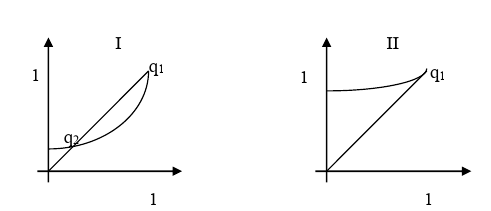
\includegraphics[width=.9\textwidth]{proc_q_vars}
    \caption{Случаи функции $ q $}
    \label{fig:proc_q_vars}
\end{figure}
